\chapter{Relay: An IR for deep learning}
\label{ch:relay}

Popular DL compiler intermediate representations (IRs) offer different tradeoffs
between expressivity, composability, and portability~\citep{
  tensorflow, pytorch_ad, chainer_learningsys2015, tangent, theano, glow}.
Extending these frameworks to accommodate
  the rapidly diversifying landscape of
  DL models and hardware platforms presents
  challenging tradeoffs between
  expressivity, composability, and portability.
Early frameworks adopted IRs
  specialized for then-state-of-the-art models and/or
  emerging hardware accelerators.
As a result, non-trivial extensions require
  patching or even forking frameworks~\citep{
    tf_fold, tf_lite, tangent, tf_eager, xla, glow, torchscript}.
Such \textit{ad hoc} extensions can improve expressivity
  while maintaining backwards compatibility with existing execution mechanisms.
However, they are difficult to design, reason about, and implement,
  often resulting in modifications that are mutually incompatible.
Nearly all popular deep learning representations were designed for
  static computation graphs, leading to numerous
  extensions designed to support dynamic neural networks.

This thesis present Relay,
  a new compiler IR for deep learning.
Relay's functional, statically typed intermediate representation (IR)
  unifies and generalizes existing DL IRs
  to express state-of-the-art models.
The introduction of Relay's expressive IR requires
  careful design of domain-specific optimizations,
  addressed via Relay's extension mechanisms.
Using these extension mechanisms,
  Relay supports a unified compiler that
  can target a variety of hardware platforms.
Relay's extensible compiler
   can eliminate abstraction overhead and
   target new hardware platforms.

Previous IRs have struggled to address these challenges, treating each
  component of the framework as a disconnected set of programming tasks.
Operators are defined in low-level languages like C++,
  connected by a dataflow graph, and then scripted
  in a host language like Python.
Consequently
  program analyses cannot cross language boundaries between components,
  inhibiting optimization and deployment.
Relay's design takes inspiration from traditional
  compiler literature where many of the challenges facing
  machine learning compilers have been well studied in the scalar setting.
We analyzed previous deep learning IRs finding ways
  to obtain the desirable properties of these IRs
  with a principled approaches, for example using references
  to split pure and in-pure fragments, or the use of closures
  to represent complex control operators.

Relay is also designed to abstract over platform specific behaviors but not prevent
  representing or optimizing for them.
Given a known target, a user can schedule a new optimization,
  and all necessary platform optimizations and code generation will occur.
Target independence might seem like a property already enjoyed widely,
  but in many frameworks each operator is implemented per platform,
  and often models only work on a single well-supported platform (i.e Nvidia GPU).
Previous IRs are either designed to be tethered to a specific end-user programming model
    or low-level operator library which enables the programs to be executed on specific platforms such as GPU.
Leveraging these features leads to powerful use cases,
  for example we are able to easily get best in class performance on many devices by mixing and matching TVM,
  with native kernel libraries to obtain the best performance, without the end user needing to adapt their program
  in anyway.
The rest of the section describes Relay’s IR and type system design, and presents some preliminary
  performance results.

We make the following contributions:
\begin{itemize}
  \item The Relay IR, a tensor-oriented, statically typed
    functional IR,
    which we describe in this chapter.
  Relay's design is motivated by the insight that functional IRs, used by
  languages from the ML family\footnote{``ML'' as in ``Meta Language,'' not
  ``Machine Learning''} can be readily adapted to support DL.
  With its \textit{expressive} semantics,
    including control flow, data structures, and first-class functions,
    Relay can represent entire state-of-the-art models.
  \item The insight that common features in ML frameworks,
    such as quantization and shape inference,
    can be reframed as standard compiler passes.
  By using this reframing we can tap into
    decades of traditional compilers research to design
    \textit{composable} optimization passes.
  \item
    A platform-agnostic representation of operators and domain specific
      optimizations which work in concert to provide \textit{portability}
      across hardware backends.
  \item
  Below we describe Relay, a tensor-oriented, statically typed,
    functional IR.
  Collections of \textit{ad hoc} extensions in previous frameworks
    that patched shortcomings in expressiveness are subsumed by a handful of well-known language
    constructs like let expressions, ADTs, first-class functions, and references.
  In addition to improving expressivity,
    incorporating these features as language constructs
    allows optimizations to more readily compose.
  \item
  By representing DL models as functional programs, we reframe traditional
    DL framework problems as compiler problems.
  Backpropagation becomes a source code transformation,
    transforming an arbitrary Relay function into its gradient function;
    \textit{ad hoc} shape inference becomes principled type inference;
    graph rewriting becomes program optimization;
    and the executor becomes (depending on what the context demands) an
    interpreter, virtual machine, or ahead-of-time compiler.
  Using this correspondence, we adapt existing
    PL techniques to the DL domain.
  \item
    A notable example of this approach is Relay's type system (Section \ref{sec:type_system}).
    Since operators have complicated semantics, shape inference is usually
      performed when shapes are fully concrete;
      however, at compile time, one does not have that luxury.
    We therefore extend a Hindley-Milner type system with type relations that encode shape
      constraints induced by operators.
    This allows Relay passes to reason about shape information at compile time.
  \item To provide portability,
    we define a platform-agnostic operator language
    and a compiler pass manager, which facilitates the development of
    passes that transform the IR to target new hardware backends.
\end{itemize}

\section{IR}

% \begin{figure}[!t]
%     \begin{jmpgrammar}
%       \bnfrule{REAL}{\real} \is{\mathbb{R}}\\
%       \bnfrule{NAT}{\nat} \is{\mathbb{N}}\\
%       \bnfrule{NAME}{\rName} \is{\texttt{(}\text{`\_'}\inlineAlt[a-zA-Z]\texttt{)}\ \
%       \atLeastZero{\text{`\_'}\inlineAlt[a-zA-Z]\inlineAlt[0-9]}}\\
%       \bnfrule{TYPE NAME}{\typename} \is{[A-Z]\ \ \atLeastZero{\text{`\_'}\inlineAlt[a-zA-Z]\inlineAlt[0-9]}}\\
%       \bnfrule{GLOBAL VAR}{\gvar} \is{\kwd{@}\rName}\\
%       \bnfrule{LOCAL VAR}{\lvar} \is{\kwd{\%} \rName}\\
%       \bnfrule{GRAPH VAR}{\graphVar} \is{\kwd{\%} \nat}\\
%       \bnfrule{TYPE VAR}{\tyvar} \is{\rName}\\
%       \bnfrule{OPERATOR}{\op} \is{\rName}\\\\
%       \bnfrule{Program}{\program} \is{\atLeastOne{\defn\inlineAlt\typedef}}
%         \alt{\expr}\\\\
%       \bnfrule{Param}{\param} \is{\rParamRule}\\
%       \bnfrule{Type Param}{\tyParam} \is{\rTyParamRule}\\\\
%       \bnfrule{Definition}{\defn} \is{\rDefnRule}\\\\
%       \bnfrule{Type Definition}{\typedef} \is{\rTypeDefRule}\\\\
%       \bnfrule{Kind}{\kind} \is{\kwd{BaseType}}
%         \alt{\kwd{Shape}}
%         \alt{\kwd{Relation}}
%         \alt{\kwd{ADT}}
%         \alt{\kwd{Type}}\\\\
%       \bnfrule{BaseType}{\basetype} \is{\kwd{int} \nat \maybe{\kwd{x} \nat}}
%         \alt{\kwd{float} \nat \maybe{\kwd{x} \nat}}
%         \alt{\kwd{bool} \maybe{\nat}}\\\\
%       \bnfrule{Shape}{\shape} \is{\kwd{(} \seq{\nat} \kwd{)}}\\\\
%       \bnfrule{Pattern}{\patt} \is[constructor]{\op \kwd{(} \seq{\patt} \kwd{)}}
%         \alt[wildcard]{\wildcard}
%         \alt[variable]{\lvar\ \maybe{\typeanno}}
%     \end{jmpgrammar}
%   \end{figure}
  \begin{figure}[t]
    % \ContinuedFloat
    \begin{jmpgrammar}
      \bnfrule{Expr}{\expr} \is[local var]{\lvar}
        \alt[global variable]{\gvar}
        \alt[constant tensor]{\kwd{const} \kwd{(} \texttt{(}\real\inlineAlt\bool\texttt{)} \kwd{,} \shape \kwd{,} \basetype \kwd{)}}
        \alt[call]{\expr \maybe{\tyargs} \args\vspace{0.2em}}
        \alt[let]{\rLetRule}
        \alt[\kwd{let}\ \kwd{\%}\_\ \kwd{=}\ \expr\kwd{;}\ \expr]{\rAnonLetRule}
        \alt[graph let]{\rGraphLetRule}
        \altSpace{0.5em}{function}{\rFnRule}
        % \altSpace{1em}{type cast?}{\kwd{(} \type \kwd{)} \expr}
        \altSpace{1em}{tuple formation}{\rTupRule}
        \alt[tuple proj.]{\rTupProjRule}
        \alt[if-else]{\rIfElse{\expr}{\expr}{\expr}}
        \altSpace{0.5em}{pattern match}{\rMatchRule}
        \altSpace{1em}{operator}{\op}
        % TODO: When will we have gradient as a first-class operator?
        % \alt[gradient]{\kwd{grad}\kwd{(}\expr\kwd{)}}
        \alt[new ref]{\kwd{ref}\kwd{(}\expr\kwd{)}}
        \alt[get ref]{\kwd{!} \expr}
        \alt[set ref]{\expr \kwd{:=} \expr}\\\\
      \bnfrule{Type}{\type} \is[base type]{\basetype}
        \alt[shape]{\shape}
        \alt[tensor type]{\kwd{Tensor} \kwd{[} \shape \kwd{,} \basetype \kwd{]}}
        \alt[type variable]{\tyvar}
        \alt[function type]{
          \begin{split}
          \kwd{fn}\ &\rTyParamsRule\\
          &\kwd{(} \seq{\type} \kwd{)}\ \rettype\\
          &\maybe{\relations}
          \end{split}
          }
        \alt[ref type]{\kwd{Ref} \kwd{[} \type \kwd{]}}
        \alt[tuple type]{\kwd{(} \seq{\type} \kwd{)}}
        \alt[type call]{\type \kwd{[} \seq{\type} \kwd{]}}
        \alt[type name]{\typename}
    \end{jmpgrammar}
    \caption{\textmd{The BNF Grammar for the \relay{} language.}}
    \label{fig:short_bnf}
  \end{figure}


The Relay IR is a high-level, functional, differentiable language.
One can understand Relay by starting from a subset of Relay
  that represents an idealized computation graph IR and
  incrementally growing to the full Relay IR.
A computation graph, in its simplest presentation, is a directed acyclic
  graph with multiple inputs and a single output.
The syntax of an equivalent computation graph is realized by
  a language with three rules (1) \verb|variable|s, (2) function \verb|call|s,
  and (3) \verb|operator|s, see Figure~\ref{fig:short_bnf} for the corresponding rules.

Relay's expressive high-level IR is designed to support
  complex models while abstracting over hardware-specific
  implementation details to enable hardware agnostic program
  analysis and optimization.
Rather than invent an entirely new language,
  Relay's IR design is based on IRs used by the well-studied ML family of
  functional programming languages (e.g., SML and OCaml).
These IRs are expressive enough to capture general-purpose programs
  (including control flow, first-class functions, and data types)
  and have clearly specified semantics (e.g., lexical scope and controlled effects).
By borrowing from PL literature,
  we can apply program analysis and optimization techniques from decades of research~\citep{haskell_vector}.

Relay's IR takes a small functional core and enriches it with domain-specific additions---namely,
  the inclusion of tensors and operators as expressions
  and a novel tensor type system design to support tensor shapes.
Our principled design
  enables the import of existing models from deep learning frameworks and exchange formats,
  the implementation of a number of domain-specific optimizations,
  and efficient deployment across a variety of targets.
In the remainder of this section,
  we describe the IR design in further detail
  and explore the ramifications of this design on the compilation stack.

The Relay IR is designed
  to subsume the functionality of computation graph-based IRs
  while providing greater faculties for abstraction, and dynamism.
We present Relay's design by incrementally building up to the full IR
  starting from a subset that corresponds to a simple computation graph.

Deep learning models fundamentally operate on tensors.
Hence, Relay's primary value type is a tensor and operators are included as language primitives
  (see the \verb|tensor constant| and \verb|operator| rules in Figure \ref{fig:short_bnf}).
Relay leaves the implementation of each operator opaque; the operators
  are represented by a lower-level IR, which is optimized independently.
A computation graph, in its simplest form, is a directed acyclic
  graph with multiple inputs and a single output.
Relay uses three constructs to support these simple graphs:
  (1) \verb|variable|, (2) function \verb|call|,
  and (3) \verb|operator|; see Figure~\ref{fig:short_bnf} for the corresponding rules.

\subsection{Operators}
...

\subsection*{Multiple Outputs}

Many common operators like \verb|split|, which splits
  a tensor along a particular axis, require multiple outputs.
In order to handle these programs,
  computation graph IRs have added primitive support
  for multiple outputs.
Multiple outputs can be modeled as tuples, which can
  be added with just two rules (1) \verb|tuple formation|
  and (2) \verb|tuple projection|.
Using a construct such a tuples cleanly handles not only multiple
  outputs but operations which return multiple aggregate values
  as a single output can also be a tuple itself.

\subsection*{Let}

By construction, computation graphs enjoy implicit sharing of subcomputations
  via multiple outgoing dependency edges.
Implicit sharing is often implemented via pointers that uniquely identify subgraphs,
  a property useful for both execution and analysis.
Previous frameworks often obtain this sharing by using a host
  language's name binding to construct a graph (e.g., by binding a Python variable
  to a subgraph and using that variable to construct other subgraphs).
General-purpose programming languages, on the other hand, provide \textit{explicit}
  sharing via binding constructs, such as \verb|let|.
In programs free of scope, ordering, and effects, implicit sharing
  and explicit sharing are semantically equivalent.
However, in practice, user programs rely on effects and ordering,
  requiring previous approaches to provide workarounds.
For example, TensorFlow's Eager Mode inserts dummy control edges
  in its generated graphs to impose effect ordering.
The lack of lexical scope in computation graphs complicates language features,
  like first-class functions and control flow,
  and reduces the precision of traditional analyses,
  such as liveness,
  because the high-level program structure is absent~\citep{funarg, funarg_sol}.
The addition of a humble \verb|let| binding, a central concept in functional languages,

\subsection*{Control Flow}

Emerging models, particularly in the domain of natural language processing, increasingly
  rely on data-dependent control flow, forcing frameworks based on computation graph IRs
  to incorporate control flow, often through \textit{ad hoc} and difficult-to-extend constructs.
For example, TensorFlow Fold~\citep{tf_fold} extends TF with special combinators that
  dynamically compute a graph for each shape permutation;
  these high-level constructs are opaque to further optimizations.
The functional programming community has demonstrated that recursion and pattern matching are sufficient
  to implement arbitrary combinators for control flow and iteration (e.g., maps, folds, and scans).
To support the definition of functional combinators
  we enrich Relay with two more language
  features to implement arbitrary combinators: \verb|if| and first-class recursive functions.

\subsection{Control Flow}

Neural networks increasingly rely on control flow, forcing frameworks based on computation graph IRs
to support this construct; however, control flow extensions are generally \textit{ad hoc}.
Even in the presence of control flow-free models, looping
  constructs are necessary to implement optimization algorithms
  such as SGD.
Furthermore emerging architectures are beginning to make greater use of
    control flow, with many architectures exposing custom control
    combinators such as loops, maps, folds, and scans.
The central challenge is a flexible and extensible encoding of
  control flow operations.
The functional programming community has demonstrated recursion and pattern matching are sufficient
  to implement arbitrary combinators for control flow and iteration.
To support the definition of functional loops we enrich Relay with two more language
  features to implement arbitrary combinators: \verb|if| and first-class recursive functions.
The guard expression in Relay's \verb|if| expression operates over rank-0 boolean tensors,
  which represent booleans.

\subsection*{First-Class Functions}

A computation graph is a single computation
  from multiple inputs to multiple outputs.
While it is tempting to reinterpret a graph as a function,
  graphs lack functional abstraction and named recursion.
The addition of first-class named functions dramatically increases
  Relay's expressivity, allowing it to encode generic
  higher-order functions and thus capture higher-level program structure.
First-class functions also enable simpler implementations
  of importers that map higher-level programs to our IR.
For example, an instance of TensorFlow's looping construct \verb|tf.while_loop|
  can be represented as a single specialized loop function
  or a generic fold over the loop state.
See Figure~\ref{fig:tf_to_relay_loop} for an example of this conversion (via
  the Relay TensorFlow frontend).

A computation graph is a single expression
  from multiple inputs (i.e. its free variables) to multiple outputs.
While it may be tempting to reinterpret a graph as a function, it lacks functional abstraction
  and named recursion.
Adding the ability to name functions and pass them as first-class values dramatically increases
  Relay's expressivity, allowing it to encode generic
  higher-order functions and readily use techniques used in functional
  compilers like automatic deforestation.
First-class functions enable passes such as
  automatic differentiation, and simplify
  the framework importers which map higher-level programs to our IR~\citep{myia}.
For example, an instance of TensorFlow's looping construct \verb|tf.while_loop|
  can be represented as a single specialized loop function
  or a generic fold over the full loop state.
See Figure~\ref{fig:tf_to_relay_loop} for an example of this conversion (via
  the Relay TensorFlow frontend).

\subsection*{Data Abstraction}
Many models make use of additional data types beyond
  tuples, such as lists, trees, and graphs~\citep{char-rnn, tree_lstm, graph_lstm}.
Relay borrows from functional languages
  a generic and principled method of extension:
  algebraic data types (ADTs).
To support them, we add mechanisms for
  (1) type declaration and
  (2) pattern matching.
This final addition results in a strict functional language,
  closely resembling the core of languages like OCaml and SML.
The increase in expressivity introduced by the Relay IR introduces
  new optimizations challenges, which we
  discuss in Chapter~\ref{ch:related}.

Earlier, we extended the language with tuples to
  emulate behavior of existing IRs.
Deep networks require additional data types like lists,
  trees, and graphs~\citep{char-rnn, tree_lstm, graph_lstm}.
Relay borrows a generic and principled way to
  extend a language with new data types:
  algebraic data types (ADTs).
To support them we add (1) a type declaration mechanism and
  (2) pattern matching.
One may question why Relay has \verb|if| when it could be subsumed by \verb|match|:
  \verb|if| is still necessary because tensors are primitives, not ADTs.
  % and thus do not have a recursion principle that characterizes their match behavior.

The resulting language is a familiar strict functional language,
  resembling the core of languages like OCaml and SML.
Our language makes domain-specific deviations from existing work,
  and we have provided a full listing
  of its syntax, operational semantics, and type rules
  in the appendix.
A functional language provides a few notable advantages.
Its pure fragment represents idealized computation graphs free
  from effects. This fragment can be easily optimized by end users who
  can reason about it as pure dataflow.
For this reason, Relay is pure by default but exposes a limited
  form of mutation via ML-style references that we have
  primarily used for automatic differentiation.

Relay is more expressive than many previous frameworks and this expressivity introduces new challenges.
  Previous essential functionality such
    as shape inference and automatic differentiation must be adapted for
    our new IR.
How does one reason about the shapes of operators when the input is unknown?
How does one backpropagate over pattern-matching, control, data types, and mutation?
In the following subsection we demonstrate how one can adapt techniques
  from type inference and checking to Relay.

% Another important semantic choice is that all Relay operators expose a functional interface, i.e they consume inputs and outputs.
% The functional semantics allow us to later introduce mutable buffers without requiring complex interprocedural program analysis.
% Our second principle was a transparent separation from the abstract representation of machine learning models, and kernels.
% The abstraction is successfully introduced by computation graph IRs, but in an opaque way which limits cross layer optimization.
% Many gestalt approaches use a single language that defines all kernels and models, requiring users to both reason about all levels during optimization.

% We are able to represent abstract operations with well known types at the Relay level via the introduction of a user extensible shape dependent
%   type system which can represent a wide range of operator’s types.

% Our final guiding principle has been target independence.
\begin{figure}[htb!]
    \begin{tabular}{ccc}
    \begin{minipage}{0.5\textwidth}
    \begin{minted}[fontsize=\small]{python}
  i = tf.constant(1)
  j = tf.constant(1)
  k = tf.constant(5)

  def c(i, j, k):
    return
      tf.equal(
        tf.not_equal(
          tf.less(i + j, 10),
          tf.less(j * k, 100)),
         tf.greater_equal(k, i + j))

  def b(i, j, k): return [i+j, j+k, k+1]

  tf.while_loop(c, b, loop_vars=[i, j, k])
    \end{minted}
    \end{minipage}
  & \hspace{-3.0em}
  \begin{Huge}
    $\Rightarrow$
  \end{Huge}
  &
    \begin{minipage}{0.5\textwidth}
    \begin{minted}[fontsize=\footnotesize]{python}
  let %while_loop =
    fn (%loop_var0: Tensor[(1,), int32],
        %loop_var1: Tensor[(1,), int32],
        %loop_var2: Tensor[(1,), int32]) {
      %0 = add(%loop_var0, %loop_var1)
      %1 = less(%0, meta[Constant][0])
      %2 = multiply(%loop_var1, %loop_var2)
      %3 = less(%2, meta[Constant][1])
      %4 = not_equal(%1, %3)
      %5 = add(%loop_var0, %loop_var1)
      %6 = greater_equal(%loop_var2, %5)
      if (min(equal(%4, %6))) {
        %9 = add(%loop_var0, %loop_var1)
        %10 = add(%loop_var1, %loop_var2)
        %11 = add(%loop_var2, meta[Constant][2])
        %while_loop(%9, %10, %11)
      } else {
        (%loop_var0, %loop_var1, %loop_var2)
      }
    }
  %while_loop(meta[Constant][3],
              meta[Constant][4],
              meta[Constant][5])
    \end{minted}
    \end{minipage}
    \end{tabular}
    \caption{
      A simple TensorFlow loop in the user-facing DSL and the Relay
        loop produced by automatically converting it.
      Note the TensorFlow while loop corresponds neatly to a tail recursive
        function.
      The Relay text format supports a ``metadata'' section which functions
        as a constant pool among other things.
      \texttt{meta[Constant][n]} represents the \texttt{n}-th constant in the
        pool.
    }
    \label{fig:tf_to_relay_loop}
    \end{figure}


\section{Type System}
\label{sec:type_system}

Relay's type system is essential
  to optimizations.
Typing guarantees both well-formedness of the program
  and provides crucial tensor shape information to perform allocation,
  check correctness, and facilitate loop optimizations.
Shape information is also valuable for data layout transformations and tensorization,
  two transformations often demanded by hardware accelerators.
In computation graph IRs, only numeric data types
  and shapes are tracked for each operator.
Symbolic shapes (i.e., shape polymorphism) are only handled
  dynamically, inhibiting certain types of optimizations.

It is possible to model arbitrarily complex static properties, such
  as shape information, with a dependent type theory~\citep{selsam_certigrad}, but such
  a design incurs significant user complexity.
By incorporating shape analysis into a broader type system,
  Relay's type system balances the desire for static tensor shapes
  with usability.
In this subsection, we describe how to extend a polymorphic type system with shape
  information and type inference with shape inference.


  Computation graph IRs rely on typing in the form of
  datatype and shape inference.
Datatype and shape inference is the process of computing the
  concrete datatypes (e.g., \verb|float32|, \verb|int32|) and shapes (e.g., $(10, 5)$, $(100, 1, 32)$) of all
  tensors in a computation graph.
Deep learning frameworks and compilers use static shape information
  to perform allocation, check correctness, and facilitate optimization.
Precise static shape information is also valuable for traditional loop
  optimizations, data layout transformations, tensorization, and
  optimizations that are necessary to map to hardware accelerators' unique ISAs.

Shape inference is usually formulated as a simple analysis over the dataflow graph that
  propagates shape information.
Shape inference looks remarkably similar to type inference.
Unlike type inference, though, shape inference is separate from the type system and
  does not provide types for functions or data structures.
Handling shape inference at compile time is desirable, because it allows optimizations to take
  advantage of this information even though certain shapes may be symbolic. Can shape information be encoded in static types?
If we type Relay as simply typed lambda calculus,
  we gain a simple system, but one that can not represent polymorphism,
  and lacks shape information.
Even with the addition of polymorphism, there is no representation of static
  shape information.
It is possible to model arbitrarily complex static properties, such
  as shape information, with dependent type theory, but such
  a design incurs significant user complexity.
Adopting a well known type system allows the application of
  classic techniques, but standard type systems do not
  provide a solution for tracking static shape information.
Relay's type system is designed to balance the desire for static tensor shapes
  without limiting the language's expressiveness.
In this subsection we describe how to extend a polymorphic type system with shape
  information and type inference with shape inference.

\begin{figure}
  \begin{footnotesize}
    \judgbox{\typecheck{\typeCtx}{\varCtx}{\expr}{\type}}{Expression $\expr$ has type $\type$ in type context $\typeCtx$ and variable context $\varCtx$.}
    \begin{inference}
    \jmpInfer{Relation-T}
       {\Delta, T_1 : \texttt{Type}, \ldots, T_n : \texttt{Type} \vdash (Rel(T_1, T_2, \ldots, T_n) \in \{ \top, \bot \}) }
       {\typecheck{\typeCtx}{\varCtx}{Rel}{\texttt{Relation}}}

    \jmpInfer{Type-Func-Def}
      {\forall{i \in [1, r]} \, \Delta; \Gamma \vdash R_i(T_1, \ldots, T_n, O) \\
       \Delta; \Gamma, a_1 : T_1, \ldots, a_n : T_n, \\
       f : \kwd{fn}( T_1, \ldots, T_n) \rightarrow O \kwd{ where } R_1, \ldots, R_r \vdash body : O}
        {\Delta; \Gamma \vdash \kwd{def @} f\kwd{(}a_1\kwd{:} T_1\kwd{,} \ldots
        a_n\kwd{:} T_n\kwd{)} \rightarrow O \kwd{ where } R_1, \ldots, R_r \kwd{ \{ } body \kwd{ \}} : \\
        \kwd{fn}(T_1, \ldots, T_n) \rightarrow O \kwd{ where } R_1, \ldots, R_r }

    \jmpInfer{Type-Call}
       {\Delta; \Gamma \vdash f : \kwd{fn} (T_1 \kwd{,} \ldots \kwd{,} T_n) \rightarrow O
         \kwd{ where } R_1, \ldots, R_r
         \\ \Delta; \Gamma \vdash a_1 : T_1, \ldots, a_n : T_n
         \\ \forall{i \in [1, r]} \, \Delta; \Gamma \vdash R_i(T_1, \ldots, T_n, O)}
       {\typecheck{\typeCtx}{\varCtx}{f(a_1, \ldots, a_n)}{O}}
    \end{inference}
  \end{footnotesize}
  \caption{Examples of Relay's typing inference rules, namely the rules for function definitions and function calls,
    where $\Delta$ is the environment for types and $\Gamma$ is the environment for variables. These demonstrate
    that type relations must hold at each call site.}
  \label{fig:partial-inference-rules}
\end{figure}


\subsection*{Tensor Types}

The primitive value in Relay is a tensor, which has
  a shape and a base type (\verb|tensor type| in Figure \ref{fig:short_bnf}).
Base types describe the elements of tensors by tracking
  the bit width,
  the number of lanes (for utilizing vectorized intrinsics),
  and whether the type is floating point or integral.
To ensure Relay can offload tensor computation to devices
  with greatly varying architectures,
  Relay tensors may only contain base types,
  preventing, for example, tensors of closures.
The shape of a tensor is a tuple of integers describing the tensor's dimensions.
A dimension may be a variable or arithmetic expression that indicates how the
  output shape of an operator depends on those of its inputs.
Functions may be polymorphic over shapes, which results
  in shape constraints that must be solved during type inference.
Sec.~\ref{sec:inference} describes the process.
Relay also supports a special shape called \verb|Any|, which is used
  to mark a dynamic shape when static relationships are not profitable
  to model.

In the context of dynamic models, many data shapes can only be determined at runtime.
Therefore, the previous assumption of static data shapes does not hold.
In order to support dynamic data shapes, Relay VM introduces a special dimension called
  Any~to represent statically unknown dimensions.
For example, we can represent a tensor type as \texttt{Tensor[(1, 10, Any), float32]},
  where the size of the third dimension in this tensor is unknown while the other
  two dimensions have concrete values.
This concept has been introduced in other frameworks.
We do not support tensor types with dynamic ranks given the relatively limited use cases and optimization opportunities.

xity.

\subsection*{Operators and Type Relations}
Operators are one of the key primitives that differs from those of
general-purpose programming languages.
Relay's use of opaque operators enables backends to choose different
lowering strategies based on the hardware target.
Relay's operator set is extensible, meaning that users may add new operations.
Supporting common or user-defined tensor operators requires a type system that can
adapt to complex shape relationships between input and output types
(e.g., elementwise operators with broadcasting semantics).

To handle the constraints between operators' argument shapes, Relay's type system
introduces type relations.
A type relation is implemented as a function in the
meta-language and represents a symbolic relationship between
the input and output types.
When developers add a new operator to Relay, they may constrain its
type with an existing relation or add their own.
Function types may include
one or more type relations over a subset of the argument types and the return type.
The type checker enforces that these relationships hold at each call site.

A difference between general purpose programming models and those tailored to deep learning
  is the use of operators as the primitive unit of computation.
The ability to add new operations to Relay requires a type system that can adapt to
  complex shape relationships between input and output types.
Many operators have types that can be defined
  as functions of the input types.
Unfortunately some are not only functions,
  but also relations that specify constraints between input and output shapes.
A key extension of Relay over traditional type systems is the addition of type relations
  to express these constraints.
When developers add a new operator to Relay, they may constrain its
  type with existing relations or add their own.
Function types (including those of operators) may include
  one or more type relations over an arbitrary subset of the argument types and the return type.
The type checker enforces that these relationships hold at the call site.
These relations may be viewed as a verification condition induced at a
  function call site, where the formula is a conjunction of the relations.
For example, primitive operators are assigned types that are universally quantified over
  both the input and output types.
We can then use a type relation to encode a constraint that must hold later
  when type checking observes specific input and output types.
Type relations are opaque in the Relay IR: they are implemented in the
  meta-language and registered when defining an operator.
However, they may be reused across different implementations.
For example, we use a relation that describes the
  broadcasting rule for all element-wise operations.


\noindent
{\bf Operator Type Relation} A type relation describes the relationship between the types of operator inputs and outputs. The type system of TVM's Relay IR relies on these type relations to infer and bidirectionally propagate type and shape relationships between inputs and outputs of operators across the whole program.
For example, the type relation for broadcasting operators (e.g. \texttt{broadcast\_add}) performs the shape calculation following the NumPy broadcasting rules\footnote{\url{https://docs.scipy.org/doc/numpy/user/basics.broadcasting.html}}.

The type relation must be generalized to properly handle dynamic shapes. For example, a program which grows a tensor on each loop iteration (a case existing in the decoder of many NLP models) is both impossible to type and compile without proper type system support. With the introduction of Any, we are able to improve the existing type relations to support dynamic models.

There are two cases that must be handled after we introduce Any~to the type relations.
First, operators such as {\tt arange}\footnote{{\tt arange} generates a range of values in a (start, stop, step) interval the arrays output size is a function of input arguments.} and {\tt unique}\footnote{{\tt unique} selects the unique elements of a tensor.} have dynamic output shapes depending on the input data, which will be described in Any.
We can now describe the type relation using the enhanced type relation functions with Any but not before.
For example, type relation of {\tt arange} can be expressed as follows
\[
arange: fn(start: fp32, stop: fp32, step: fp32) \rightarrow \langle [Any], fp32 \rangle
\]
Second, when input shapes of a type relation contain Any~dimension, the type relation needs to propagate Any~correctly to the output types and relax typing constraints that hold in the static cases when necessary.
For example, type relation for {\tt broadcasting} operators determines the compatibility between corresponding
dimensions from both inputs if they are equal or one of them is 1 according to the Numpy broadcasting rule.
For example, the rules
for broadcast type relation given the matching dimension from two inputs when having Any~are defined as follows:
\begin{align*}
  \textrm{broadcast\_rel}(Any, 1) &\rightarrow Any \\
  \textrm{broadcast\_rel}(Any, d) &\rightarrow d ~~~~~~(d > 1) \\
  \textrm{broadcast\_rel}(Any, Any) &\rightarrow Any.
\end{align*}
Note that due the presence of dynamic shapes these type relation rules can no longer rule out all type errors at compile-time.
For example, for the second rule shown above, when Any~is neither 1 nor $d$ at runtime, it then violates the broadcast type constraints.
To address this, we take the gradual typing~\citep{gradualtyping} approach and leave certain type checking at runtime after Any~is instantiated by a
concrete value (see \autoref{sec:compilation:shape-func} for more details).
One could eliminate these errors using a more advanced type system, but at increased complexity.

\section{Type Inference}
\label{sec:inference}

The most interesting parts of the type system
are where shape computation occurs.
We highlight a few examples of Relay's inference
rules in Fig.~\ref{fig:partial-inference-rules};
the full typing rules can be found in the appendix.
In this subsection we focus on design decisions behind Relay's type system
and the implementation of type inference.
To incorporate type relations into Relay's type system, we enrich
a Hindley-Milner type inference algorithm with
a constraint solver for type relations.
Relay's inference algorithm has three steps: first it
performs a pass over the AST generating types (potentially involving type variables)
as well as populating the set of relations,
then it solves the incurred constraints,
and finally it assigns types to each expression in the AST.
A type relation is implemented as a function in the
meta-language and represents the symbolic relations between
the input and output types of an object-language function.
When the type inference algorithm visits a function call site, the function's type relations are
instantiated to the types at the call site and added to a queue of relations waiting to be
solved.
The relationships between the call's type variables and its relations are are added to a
bipartite undirected dependency graph where the two disjoint sets are type variables and type relations.
Traditional unification constraints are represented using a modified union-find structure that
integrates with the dependency graph.

Once the queue is populated, the algorithm will dequeue a relation and attempt to solve it.
There are two cases when solving a type relation:
\begin{enumerate}
\item If all the relation's type variables
are concrete, we call the type relation function. If that function returns true, the
constraint is discharged. Otherwise, type checking fails.
\item If any type is fully or partially symbolic, the
  algorithm will propagate
  existing concrete type information via unification.
All relations affected by new assignments to type
  variables (as determined by the dependency graph)
  are moved to the beginning of the queue.
If the current type relation is now completely solved, we
discard it to avoid unnecessarily visiting it again.
\end{enumerate}

Our fine-grained dependence graph provides the transitive dependencies
between relations and unification variables.
The use of fine-grained dependencies enables our algorithm to
only retry a minimal number of relations when we
learn a new variable assignment.
We run this to fixpoint or until the queue is empty.
If the queue is not empty and no progress is made between iterations,
then at least one variable is under constrained and inference fails.
Note that a type relation's implementation can
compromise type soundness, as they are axiomatic descriptions
of operations implemented outside of Relay.
Luckily, in practice, the number of type relations needed to express most of Relay's
operators is relatively small, and their implementations are generally straightforward
and amenable to exhaustive testing.
The above sections discuss the core of Relay, a full-length paper under submission\citep{roesch2019relay}
details its design and implementation.

To incorporate type relations into Relay's type system, we enrich
a Hindley-Milner-style type inference algorithm with
a constraint solver.
Relay's inference algorithm has three steps: first, it
performs a pass over the AST, generating types and a set of relations,
then it solves the incurred constraints,
and finally annotates each sub-expression with its inferred type.

% a queue of relations. dequeue a relation and attempt to solve it by invoking it's opaque
% type-relation function.
% 1. all type variables concrete & relationship holds => solved. discard relation
% 2. all type variables concrete & relationship doesn't hold => type error
% 3. types are partially symbolic => propagate unif. constraints to its inputs and output. if
% all type variables are solved/assigned/concrete, discard relation. otherwise add it and the
% relations that depend on the solved variables to queue. those that are already on the queue should
% be reprioritized

When the type inference algorithm visits a function call site, the function's type relations are
instantiated with the concrete argument types at the call site.
Each instantiated relation is added to the queue of relations to solve.
The relationship between a call's type variables and relations is added as an edge to
a bipartite dependency graph where the two disjoint sets are type variables and type relations.
Traditional unification constraints are represented using a modified union-find structure that
integrates with this dependency graph.

Once the queue is populated, the algorithm will dequeue a relation and attempt to solve it.
There are two cases when solving a type relation:
\begin{enumerate}
\item If all the relation's type variables
are concrete, we the relation function. If that function returns true, the
constraint is discharged. Otherwise, type checking fails.
\item If any type is fully or partially symbolic, the
  algorithm will propagate
  existing concrete type information via unification.
All relations affected by new assignments to type
  variables (as determined by the dependency graph)
  are moved to the beginning of the queue.
If the current type relation is now completely solved, we
discard it to avoid unnecessarily visiting it again.
\end{enumerate}

We run this to fixpoint or until the queue is empty.
If the queue is non-empty and no progress is made between iterations,
then at least one variable is underconstrained and inference fails.
Note that a type relation's implementation can
compromise type soundness, as they are axiomatic descriptions
of operations implemented outside of Relay.
In practice, the number of type relations needed to express Relay's
operators is small, and their implementations are straightforward
and amenable to exhaustive testing.

To incorporate type relations into Relay's type system, we enrich
  a Hindley-Milner-style type inference algorithm with
  a constraint solver.
Relay's inference algorithm has three steps: first, it
  performs a pass over the AST, generating types and a set of relations,
  then it solves the incurred constraints,
  and finally annotates each sub-expression with its inferred type.

% a queue of relations. dequeue a relation and attempt to solve it by invoking it's opaque
% type-relation function.
% 1. all type variables concrete & relationship holds => solved. discard relation
% 2. all type variables concrete & relationship doesn't hold => type error
% 3. types are partially symbolic => propagate unif. constraints to its inputs and output. if
% all type variables are solved/assigned/concrete, discard relation. otherwise add it and the
% relations that depend on the solved variables to queue. those that are already on the queue should
% be reprioritized

When the type inference algorithm visits a function call site, the function's type relations are
  instantiated with the concrete argument types at the call site.
Each instantiated relation is added to the queue of relations to solve.
The relationship between a call's type variables and relations is added as an edge to
  a bipartite dependency graph where the two disjoint sets are type variables and type relations.
Traditional unification constraints are represented using a modified union-find structure that
  integrates with this dependency graph.

Once the queue is populated, the algorithm will dequeue a relation and attempt to solve it.
There are two cases when solving a type relation:
\begin{enumerate}
  \item If all the relation's type variables
  are concrete, we the relation function. If that function returns true, the
  constraint is discharged. Otherwise, type checking fails.
  \item If any type is fully or partially symbolic, the
    algorithm will propagate
    existing concrete type information via unification.
  All relations affected by new assignments to type
    variables (as determined by the dependency graph)
    are moved to the beginning of the queue.
  If the current type relation is now completely solved, we
  discard it to avoid unnecessarily visiting it again.
\end{enumerate}

We run this to fix-point or until the queue is empty.
If the queue is non-empty and no progress is made between iterations,
  then at least one variable is unconstrained and inference fails.
Note that a type relation's implementation can
  compromise type soundness, as they are axiomatic descriptions
  of operations implemented outside of Relay.
In practice, the number of type relations needed to express Relay's
  operators is small, and their implementations are straightforward
  and amenable to exhaustive testing.

One caveat of the Any~dimension is that unknown dimensions will
  propagate during type inference, reducing chances for shape specialization.
For example, if we use an operator such as {\tt arange} to produce a
  tensor with dynamic shape (i.e., \texttt{Tensor[(Any,), float32]})
  and later {\tt broadcast\_add} to a tensor with static shape (i.e., \texttt{Tensor[(5, 1), float32]}),
  the output shape will also contain an Any~dimension (i.e., \texttt{Tensor[(5, Any), float32])}.

To limit the contamination of Any, we further introduce {\em sub-shaping}
  to improve the precision of types computed by type-inference.
Much like sub-typing used in popular programming languages \citep{LiskovTPLS1994,AmadioAmadioTPLS1993},
  our extension enables values with more specific shape information to be passed in contexts which require less specific shapes.
Further, we perform extra analysis that repeatedly replace one Any~dimension by a symbolic variable followed by
  a type inference pass to identify if other Any~dimensions share the same symbolic expression.
%on each Any~dimension to detect if two Any~dimensions point to an identically sized dimension.
This information is passed to downstream compilation
  and can reduce the search space during the symbolic codegen.
We can use this analysis in the downstream compilation
  to generate shape-specialized code during codegen.

We treat concrete dimension and symbolic dimension as a sub-shape of Any.

Rules for invoking a function, suppose fn type is $fn\langle T_1, \dots, T_n\rangle$,
and arguments are $T'_1, \dots, T'_n$, the rules are defined as follows
\begin{align*}
  \textrm{union}(T_i, T'_i) &\rightarrow T_i \\
  \textrm{join}(T_i, T'_i) &\rightarrow T'_i
\end{align*}

\subsection{Shape Function}
\label{sec:type_systemTech:shape-func}
Existing deep learning compilers only deal with static shapes,
  enabling all shape computation to occur at compile-time.
Therefore, it is easy to allocate memory for the tensors
  using static shape information to compute the precise amount of storage needed for each tensor.
However, introducing Any~invalidates this pre-allocation
  mechanism as the tensors may now contain dynamic dimensions.
The introduction of Any~dimension invalidates the pre-allocation
  mechanism adopted in the existing deep learning compiler.
Instead, we now have to track the amount of memory required to be allocated in parallel to computing.
Furthermore, static type checking cannot eliminate all
  type errors at compile-time due to dynamic tensor shapes.
Consequently, we define a {\em shape function} to compute the output shape
  for storage allocation and verify the type relation in accord with the semantics of every operators.
The shape function is similar in structure to the type relations described in
  \ref{sec:type_system} but are present at runtime instead of compile-time.
The shape function enables compiling and embedding the computation of output shapes into the program.

According to the characteristics of the operator, we divide the shape functions
  in three different modes: data independent, data dependent, and upper bound.
\begin{itemize}
  \item {\em Data independent} shape functions are used for operators in which the output shape
        only depends on the shapes of inputs such as normal 2-D convolution.
  \item {\em Data dependent} shape functions require the concrete input values to compute the output shapes.
        For example, the output shape of \texttt{arange} depends on the value of start, stop, and step.
  \item In addition, there are certain operators such as Non Maximum Suppression (\texttt{nms}) where the
        complexity of computing the output shapes is on par with the complexity of executing the operator itself.
  In order to avoid the redundant computation, we use an {\em upper bound} shape function to quickly estimate an upper bound shape for the output.
  We also require such operators to return the output shape along with output value, so as to use the real shape to slice the output tensors into precise output shape and layout.
\end{itemize}

It is worth noting that in the presence of dynamic shape functions,
  operator fusion needs to be specially taken care of.
However, we only define the shape function at elementary operator level.
As a result, we also must fuse shape functions in parallel with the operator fusion.
The compiler can easily connect the shape functions of basic operators to form the shape
  function for a composite operator when all shape functions are data independent.
However, a basic operator with a data dependent or upper bound shape function cannot be fused to other operators,
  i.e., taking the outputs of other operators as its inputs to fuse together,
  as the shape function requires to access to the intermediate result within a composite operator.
As a result, we explicitly define the fusion policy to prevent this from happening.
If all basic ops in a composite op have data independent shape functions,
  it is straightforward to generate shape function for this composite op
  as we can just connect the shape functions of basic ops together.
However, a composite op is invalid if a basic op that has a data dependent
  or upper bound shape function takes the intermediate output of another basic op as input.
Because the intermediate result in a composite op is inaccessible from outside,
  the data dependent shape function cannot collect all arguments it required.
Thus, we revise the operator fusion policy correspondingly to make sure
  composite ops generated by the operator fusion pass will be valid.

Due to our definition of shape functions we are able to perform fusion
  using a generalized version of the algorithm used for standard operator fusion
  which handles passing the appropriate input shape or input depending on the shape function.
For example imagine that the fuse operator has a single input that was originally
  used an operator that requires the input, and the second fused operator requires the input shape.
Depending on the type of the shape function defined above, we handle operator fusion in the following manner.
Any data independent shape functions could be fused with other operators.
Any fused group can only have at most one shape function and it should be fused together with the operator that needs shape function.

\section{Evaluation}
\label{sec:eval}

We evaluated Relay on several systems (x86 CPUs, ARM CPUs, NVIDIA GPUs, Xilinx FPGAs) and over
  diverse vision and NLP workloads to demonstrate that (1) Relay enables \emph{composability} of
  graph-level optimizations, (2) Relay delivers \emph{performance} on inference tasks competitive
  with state-of-the-art frameworks (TensorFlow, PyTorch, MxNet), and (3) Relay provides
  \emph{portability} over difficult-to-compile-to hardware backends such as FPGAs

\subsection{Relay: A high-level IR for Deep Learning}
  In particular, our evaluation is composed of three parts:
  \begin{enumerate}
    \item \textbf{Relay enables composable optimizations}: Relay
      supports composing program transformations into multiple optimization tiers.
    \item \textbf{Relay provides competitive performance}: Despite increasing
      expressiveness, Relay's performance is competitive with the
      state of the art on popular models.
    \item \textbf{Relay handles challenging backends}: Relay can compile
      models to execute efficiently on a variety of
      backends, such as FPGA accelerators, which require quantization, layout
      optimizations, and bit-packing transformations.
    \item \textbf{Relay supports expressive models}: It can compile models with complex control flow
      like Char-RNN to a single lean binary, beating PyTorch inference performance by up to 3x.
  \end{enumerate}

  We evaluated the following vision models:
    \textit{Deep Q-Network (DQN)}, a DNN that achieved state-of-the-art performance
    on 49 Atari games in 2015;
    \textit{MobileNet}, a DNN designed for image recognition on mobile and
    embedded devices;
    \textit{ResNet-18}, a DNN for image recognition that achieved state-of-the-art
    performance on ImageNet detection tasks in 2015;
    \textit{VGG-16} (named for the Visual Geometry Group
    at Oxford), a CNN used for image recognition tasks
    \citep{dqn, mobilenet, resnet, vgg}.

  We evaluated the following NLP models:
    \textit{CharRNN}, a generator character-level
    RNN from a PyTorch tutorial;
    \textit{TreeLSTM}, a generalization of LSTMs to
    tree-structured network topologies;
    \textit{RNN, GRU, and LSTM}, a selection of models from the Gluon
    model zoo
    \citep{pytorch_rnn_tut, tree_lstm, gluon_model_zoo}.

\subsection{Experimental Methodology}
  Because we only evaluate inference in this paper,
    we frequently make use of random inputs to models when measuring
    performance.
  There were two exceptions where we evaluated on real data because
    it was readily available: CharRNN and TreeLSTM.

  For models where the input is random,
    we run 1000 timed iterations.
  Before the timed runs,
    we run 8 untimed ``warm-up'' iterations to ensure any caching and JIT compilation
    employed in lower levels of the stack are included in the 1000 timed runs.
  This way,st
    the timed runs reflect the \textit{stable} performance of the system.
  For our purposes, ``performance'' refers to end-to-end framework time on
    inference tasks (i.e., the time it takes to run a trained model) in a
    single-machine setting.

  Our vision experiments from Chapter~\ref{ch:related} and Section~\ref{sec:perf-gpu} were run on a machine with an AMD Ryzen
    Threadripper 1950X 16-Core CPU,
    an NVidia 1080 Ti GPU,
    and 64 GB of RAM.
  Our NLP experiments from Section~\ref{sec:perf-gpu} were run on a machine with an AMD Ryzen
    Threadripper 1950X 16-Core CPU,
    an NVidia Titan-V GPU,
    and 64 GB of RAM.
  Our low-power vision experiments from Section~\ref{sec:low-power} were run on multiple edge-class ARM development boards: a RaspberryPi 3, a Firefly RK3399, and an Ultra-96 FPGA platform.
  We evaluated Relay's handling of accelerators on a VTA design with a
    $16\times16$ matrix-vector 8-bit tensor core clocked at 333MHz on the Ultra-96 platform.

  In terms of software, we used
    Cuda version 10.0,
    CuDNN version 7.5.0,
    TVM commit \texttt{cefe07e2a}\footnote{NLP experiments required custom modifications that may be made public later},
    MxNet version 1.4.0,
    Pytorch version 1.0.1post2,
    and TensorFlow version 1.13.1.

  The Relay vision experiments utilized aggressively tuned TVM schedules on the GTX 1080 Ti GPU,
    improving performance significantly.

  \subsection{Relay Provides Competitive Performance}
  \label{sec:perf-gpu}

  \begin{figure}[h]
    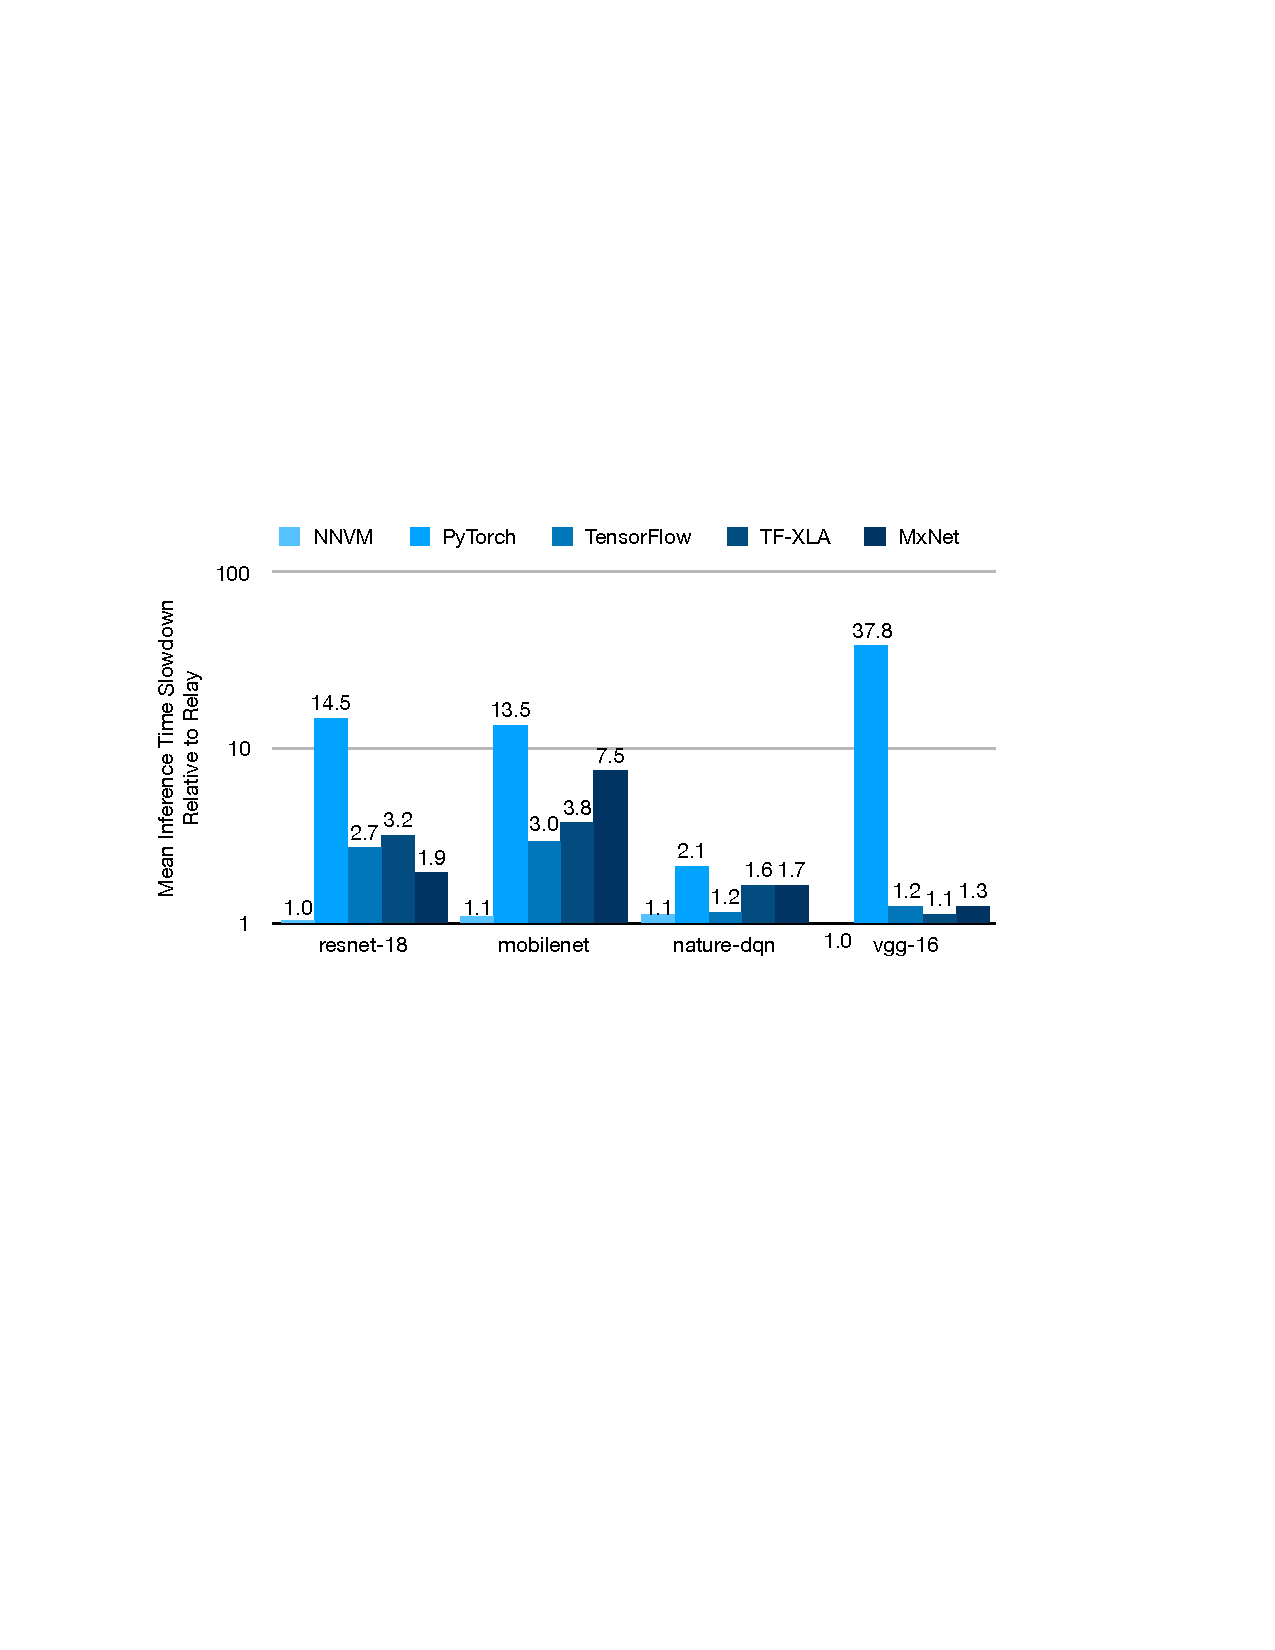
\includegraphics[width=
    \textwidth]{fig_splash19/eval/vision_1080Ti_relay.pdf}
    \caption{
      Inference slowdown of popular frameworks relative to Relay on vision
        benchmarks running on NVIDIA GTX 1080 Ti GPUs.
      Relay provides performance competitive to the state of the art.
      We ran 1000 trials for each model and used the AoT compiler.
    }
    \label{fig:vision-eval}
  \end{figure}

  \begin{figure}[h]
    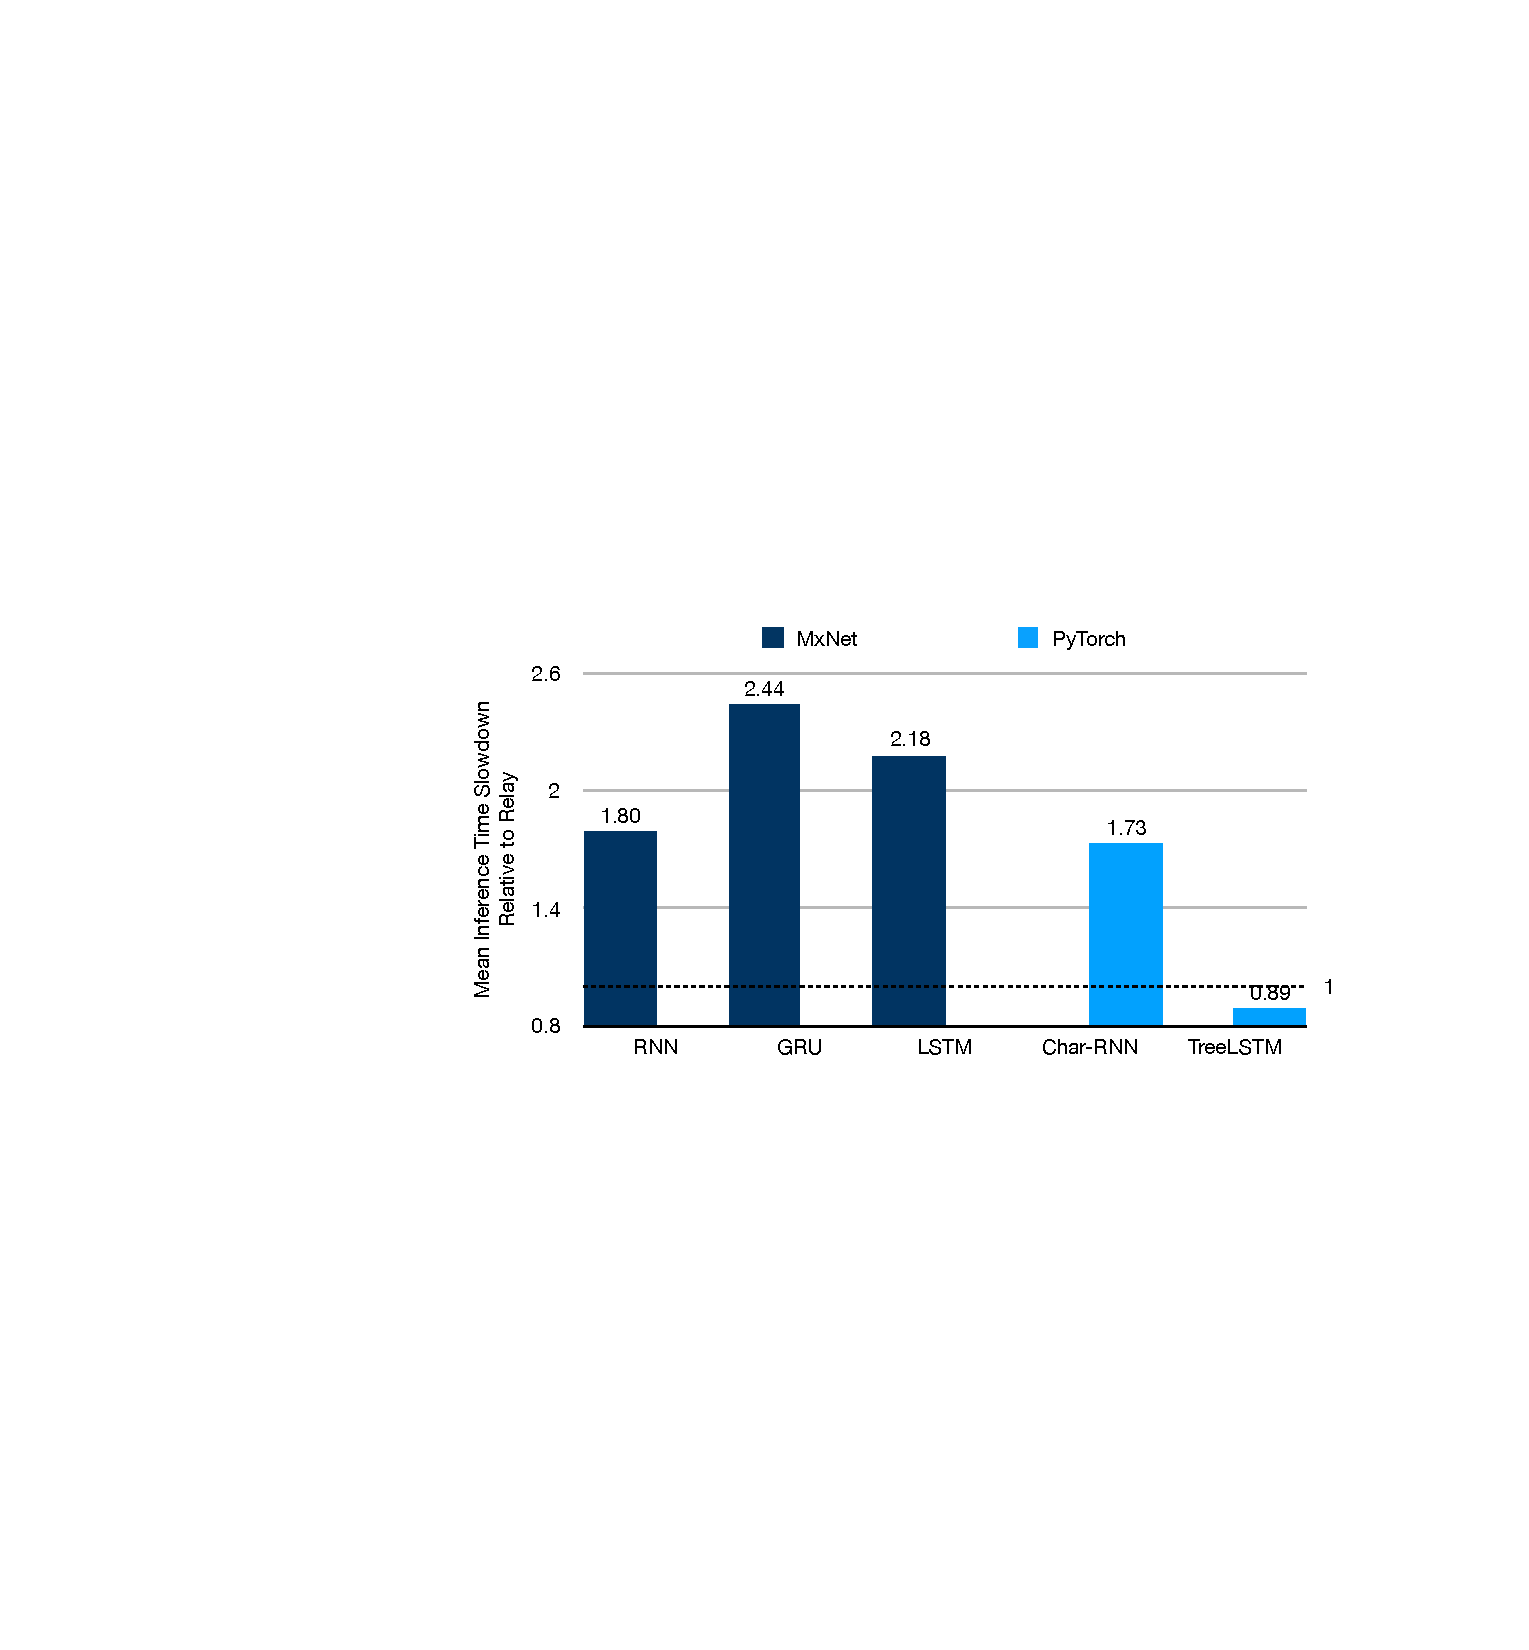
\includegraphics[width=
    \textwidth]{fig_splash19/eval/nlp_TitanV_relay.pdf}
    \caption{
      Inference slowdown relative to Relay on NLP benchmarks running on NVIDIA
        Titan-V GPUs.
      NLP workloads feature control flow,
        which makes them more challenging to optimize.
      Relay provides performance competitive to state of the art (up to
        2.4$\times$ speedup over MxNet on GRU).
      We ran 1000 trials for each model, except for CharRNN, on which we used 100 trials.
    }
    \label{fig:nlp-eval}
  \end{figure}

  An age-old story in compilers literature is that increasing expressivity
    impacts the global performance of the system.
  We set out to build zero-cost abstractions for Relay,
    governed by Stroustrup's principle, ``What you don't use, you don't pay
    for'' \citep{bjarne}.
  We demonstrate that we can achieve competitive performance on both CPUs and
    GPUs on a wide set of CNNs that are well supported by existing frameworks.
  We evaluated inference time for two classes of workloads: computer vision and natural language processing.
  We compared Relay (using our AoT compiler) to \nnvm,
    TensorFlow, TensorFlow-XLA (Accelerated Linear Algebra), PyTorch, and MxNet.
  We ran the vision and NLP workloads on GTX 1080 Ti and Titan-V GPUs, respectively.

  \subsection{Vision Evaluation}
  % Figure~\ref{fig:vision-eval} compares Relay against state of the art frameworks
  %   running vision workloads on a GTX 1080 Ti GPU.
  We ran each model with
    batch size 1, a common setting in inference tasks.
  Relay achieves performance on par with \nnvm,
    an existing deep learning graph compiler in use at Amazon.
  Relay outperforms TensorFlow, TensorFlow-XLA, MxNet and
    PyTorch on every benchmark.
  Relay's ability to do aggressive optimizations like operator
    fusion on long chains of operations, generating hardware
    specific implementations, enables it to outperform
    existing frameworks that don't perform inter-operator optimizations.

  \subsection{NLP Evaluation}
  % Figure~\ref{fig:vision-eval} compares Relay against state-of-the-art NLP models on a Titan-V GPU.
  % Implementations of the NLP models were not available in all frameworks;
    we used MxNet baselines for RNN, GRU, and LSTM and PyTorch for Char-RNN and TreeLSTM.
  % We ran the models for 1000 iterations per input, except char-RNN, which we ran for 100 ???.
  % To run the RNN, GRU, and LSTM benchmarks in MxNet, and Char-RNN, and TreeLSTM
  %   in PyTorch.
  Relay performs better than MxNet on recursive models
    due to the fact they are implemented in Python using
    MxNet's looping constructs.
  PyTorch instead uses handwritten and heavily optimized
    C implementations of the recursive network cells.
  Due to this we perform slightly \emph{worse} than PyTorch.
  It is interesting to note that our pure Relay
    implementation performs competitively against
    the hand-optimized version.

  \subsection{Targeting Deep Learning Accelerators on FPGAs}

  \begin{figure}[h]
    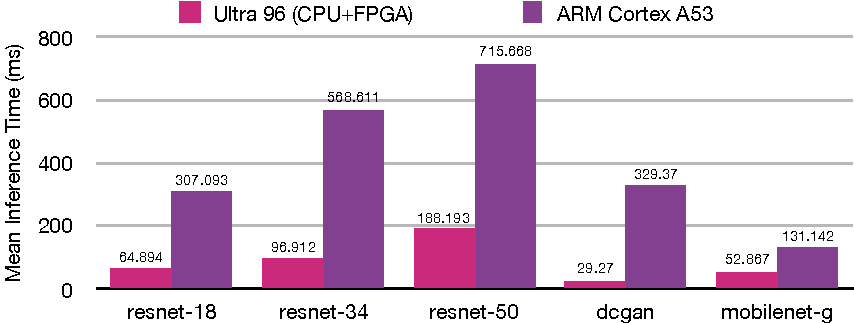
\includegraphics[width=\textwidth]{fig_splash19/eval/vision_fpga.pdf}
    \caption{
      Inference time (ms) of vision DNNs on Ultra-96 FPGA-enabled SoC.
      We compare vision workloads that Relay compiles onto the embedded Cortex
        A53 CPU vs. a DNN accelerator implemented on the integrated FPGA fabric.
      Targeting DNN accelerators can unlock up to 11x speedups, but requires a
        multitude of graph-level transformations.
      We used 10 trials for each model.
    }
    % \label{fig:fpga-eval}
  \end{figure}

  We evaluated inference time on five models including MobileNet-G \citep{mobilenet}, a grouped variant of the MobileNet architecture; ResNet-18, ResNet-34, and ResNet-50\citep{resnet}; and Deep Convolutional Generative Adversarial Networks \citep{dcgan}, a generative DNN used in unsupervised learning.
  Overall, Relay helps us efficiently offload deep learning operators onto specialized accelerators like VTA.
  Our results in Figure~\ref{fig:fpga-eval} show that we can achieve between 2.5 to 11.7$\times$ reduction in single-batch inference latency by offloading critical operators to the FPGA accelerator.
  These experiments demonstrate Relay's ability to target current and future deep learning architectures:
  \begin{enumerate}
    \item \textit{Heterogeneous FPGA/CPU offloading}: Relay lets us define the rules for offloading specific operators to the FPGA-based accelerator.
    \item \textit{Push-button quantization}: Relay can take a \texttt{fp32} model and convert its parameters to \texttt{int8} in order to enable inference on specialized accelerators.
    \item \textit{Accelerator-friendly data packing:} Relay reorganizes data so it can be effortlessly consumed by a specialized TPU-like accelerator~\citep{tpuv1}.
  \end{enumerate}

The scenario presented in the introduction demonstrates the three-pronged \textbf{extensibility challenge}
  for DL IRs:
% \begin{enumerate} % [label=\arabic*.]
%   \item \textit{Expressivity}: It should be straightforward to write models involving complex data structures (e.g., trees, graphs, and lists) and control flow.
%   \item \textit{Composability}: It should be straightforward to add and compose new optimizations
%     with existing ones (e.g., quantization, operator fusion, and automatic differentiation).
%   \item \textit{Portability}: It should be straightforward to add new hardware backends
%     (e.g., TPU, Inferentia, and FPGAs)~\citep{tpuv1, inferentia}.
% \end{enumerate}

